\documentclass[11pt]{article}

% Paquetes
\usepackage[utf8]{inputenc}
\usepackage[T1]{fontenc}
\usepackage[spanish]{babel}
\usepackage{hyperref}
\usepackage{graphicx}
\usepackage{booktabs}
\usepackage{longtable}
\usepackage{enumitem}
\usepackage{geometry}
\geometry{margin=1in}
\usepackage{tabularx}
\usepackage{array}

% Información del documento
\title{Documentación del Proyecto UPINION}
\author{Ricardo Emmanuel Uriegas Ibarra - 2230122 \\ Angel Ivan Cabrera Rojas - 2230343 \\ Alexis Guadalupe Medina Ayala - 2130234}
\date{\today}

\begin{document}

\maketitle
\tableofcontents
\newpage

\section{Descripción General}

\textbf{Objetivo:} \\
Desarrollar una aplicación web en la que los alumnos de la UPV puedan calificar de forma anónima a sus profesores, utilizando una escala de 1 a 5 estrellas. La aplicación permitirá recopilar las calificaciones para generar estadísticas y ayudar a mejorar la calidad de la enseñanza.

\bigskip
\textbf{Público objetivo:} \\
Estudiantes de la UPV que deseen expresar su opinión sobre la labor de sus profesores de manera anónima.

\newpage
\section{Visión del Proyecto}

El proyecto \textbf{CalificaProf-UPV} tiene como objetivo principal crear una plataforma web en la que los alumnos de la UPV puedan expresar su opinión sobre la labor de sus profesores de manera anónima. La visión del proyecto es la siguiente:

\begin{itemize}
    \item \textbf{Transparencia y Mejora Continua:} Facilitar un medio para que los estudiantes proporcionen feedback honesto y constructivo, permitiendo a la institución y a los profesores conocer áreas de oportunidad y fortalezas en la enseñanza.
    \item \textbf{Accesibilidad y Usabilidad:} Ofrecer una interfaz intuitiva y responsiva, que permita a los usuarios acceder y utilizar la aplicación desde cualquier dispositivo, sin complicaciones.
    \item \textbf{Análisis de Datos:} Recopilar y analizar las calificaciones y comentarios para generar estadísticas y reportes que sirvan de base para la toma de decisiones en la mejora de la calidad educativa.
    \item \textbf{Privacidad y Seguridad:} Garantizar el anonimato de los estudiantes al momento de calificar, protegiendo la integridad de los datos y promoviendo un ambiente seguro y confiable.
\end{itemize}

\newpage
\section{Requisitos del Usuario}

Para que la aplicación cumpla con las expectativas de sus usuarios, se han identificado los siguientes requisitos:

\subsection*{Requisitos Funcionales}
\begin{itemize}
    \item Permitir a los alumnos ver el listado completo de profesores.
    \item Facilitar el acceso a la información básica de cada profesor (nombre, departamento, foto).
    \item Proveer una interfaz para calificar a cada profesor utilizando una escala de 1 a 5 estrellas.
    \item Permitir la opción de agregar un comentario de manera opcional junto a la calificación.
    \item Mostrar estadísticas agregadas de las calificaciones (calificación promedio, número total de evaluaciones, etc.).
\end{itemize}

\subsection*{Requisitos No Funcionales}
\begin{itemize}
    \item La aplicación debe ser fácil de usar y accesible desde dispositivos móviles y de escritorio.
    \item Garantizar el anonimato de las calificaciones, de forma que ningún alumno pueda ser identificado.
    \item La plataforma debe responder de manera rápida ante las interacciones del usuario.
    \item El diseño debe ser claro y amigable, promoviendo una experiencia de usuario satisfactoria.
\end{itemize}

\newpage
\section{Análisis de Visibilidad}

El análisis de visibilidad tiene como objetivo definir quiénes son los stakeholders del proyecto y cómo se visualizarán los resultados de las evaluaciones en la plataforma. Se destacan los siguientes aspectos:

\begin{itemize}
    \item \textbf{Usuarios Directos:} 
    \begin{itemize}
        \item \textbf{Estudiantes:} Utilizarán la plataforma para calificar de forma anónima a sus profesores y conocerán las estadísticas generales de las calificaciones.
        \item \textbf{Administradores:} Supervisarán el correcto funcionamiento de la plataforma, gestionarán reportes y garantizarán la integridad de los datos.
    \end{itemize}
    \item \textbf{Resultados Públicos:} 
    \begin{itemize}
        \item Se mostrará un panel de estadísticas donde se visualizará la calificación promedio de cada profesor, junto con la distribución de las evaluaciones.
        \item La visibilidad de los datos se limitará a información agregada, manteniendo el anonimato de las evaluaciones individuales.
    \end{itemize}
    \item \textbf{Accesibilidad de la Información:} 
    \begin{itemize}
        \item La plataforma dispondrá de un diseño responsivo, asegurando que la información sea fácilmente visible y navegable en distintos dispositivos.
        \item Se implementarán filtros y opciones de búsqueda para facilitar a los usuarios la consulta de la información deseada.
    \end{itemize}
    \item \textbf{Confidencialidad y Seguridad:} 
    \begin{itemize}
        \item Se aplicarán mecanismos de seguridad para proteger los datos y garantizar el anonimato de los usuarios.
        \item El acceso a información sensible se restringirá a los administradores mediante autenticación y control de accesos.
    \end{itemize}
\end{itemize}


\newpage
\section{Pantallas (Wireframes/Mockups)}

Debido a la naturaleza del proyecto, se han definido las siguientes pantallas:

\subsection{Pantalla de Inicio}
\begin{itemize}
    \item Breve introducción al funcionamiento de la aplicación.
    \item Acceso a la sección de calificaciones sin necesidad de registro (la identidad permanece anónima).
\end{itemize}

\subsection{Pantalla de Listado de Profesores}
\begin{itemize}
    \item Visualización de una lista de profesores disponibles para calificar.
    \item Filtros de búsqueda (por departamento, nombre, etc.).
\end{itemize}

\subsection{Pantalla de Detalle y Calificación del Profesor}
\begin{itemize}
    \item Información básica del profesor (nombre, departamento, foto, etc.).
    \item Sistema de calificación: opción para seleccionar entre 1 y 5 estrellas.
    \item Opción para dejar un comentario opcional.
    \item Botón para enviar la calificación.
\end{itemize}

\subsection{Pantalla de Estadísticas y Resultados}
\begin{itemize}
    \item Visualización de la calificación promedio de cada profesor.
    \item Gráficos o tablas que muestren la distribución de las calificaciones.
\end{itemize}

\subsection{Pantalla de Ayuda/Soporte}
\begin{itemize}
    \item Información sobre el uso de la plataforma.
    \item Preguntas frecuentes y contacto para soporte.
\end{itemize}

\newpage
\section{Recursos Funcionales y No Funcionales}

\subsection{Requisitos Funcionales}
\begin{itemize}
    \item \textbf{Calificación Anónima:}
    \begin{itemize}
        \item Permitir a los alumnos calificar a los profesores sin identificar al usuario.
        \item La calificación debe ser de 1 a 5 estrellas.
    \end{itemize}
    \item \textbf{Visualización de Profesores:}
    \begin{itemize}
        \item Mostrar un listado de profesores con opción de búsqueda y filtrado.
    \end{itemize}
    \item \textbf{Detalle del Profesor y Calificación:}
    \begin{itemize}
        \item Permitir ver la información básica del profesor y enviar una calificación.
        \item Posibilidad de dejar un comentario opcional.
    \end{itemize}
    \item \textbf{Estadísticas:}
    \begin{itemize}
        \item Calcular y mostrar la calificación promedio y la distribución de las calificaciones.
    \end{itemize}
\end{itemize}

\subsection{Requisitos No Funcionales}
\begin{itemize}
    \item \textbf{Seguridad y Privacidad:}
    \begin{itemize}
        \item Garantizar el anonimato de los alumnos al realizar las calificaciones.
        \item Proteger la integridad de los datos.
    \end{itemize}
    \item \textbf{Usabilidad:}
    \begin{itemize}
        \item Interfaz sencilla e intuitiva.
        \item Diseño responsivo para uso en dispositivos móviles y de escritorio.
    \end{itemize}
    \item \textbf{Rendimiento:}
    \begin{itemize}
        \item Respuesta rápida en la carga de profesores y envío de calificaciones.
    \end{itemize}
    \item \textbf{Mantenibilidad:}
    \begin{itemize}
        \item Código modular y bien documentado para facilitar futuras actualizaciones.
    \end{itemize}
\end{itemize}

\newpage
\section{Documentación Técnica}

\subsection{Arquitectura del Sistema}
\begin{itemize}
    \item \textbf{Frontend:}
    \begin{itemize}
        \item Aplicación web desarrollada con tecnologías modernas (por ejemplo, React.js, Angular o Vue.js).
    \end{itemize}
    \item \textbf{Backend:}
    \begin{itemize}
        \item API REST para gestionar la obtención de la lista de profesores, envío de calificaciones y consulta de estadísticas.
        \item Tecnologías sugeridas: \texttt{Node.js}, \texttt{Django} o \texttt{Flask}.
    \end{itemize}
    \item \textbf{Base de Datos:}
    \begin{itemize}
        \item Sistema relacional (MySQL, PostgreSQL) para almacenar la información de los profesores y las calificaciones.
    \end{itemize}
    \item \textbf{Servicios Adicionales:}
    \begin{itemize}
        \item Integración de herramientas para visualización de datos (por ejemplo, Chart.js o D3.js) en la sección de estadísticas.
    \end{itemize}
\end{itemize}

\subsection{Casos de Uso Principales}
\begin{itemize}
    \item \textbf{CU1 – Visualización de Profesores:}
    \begin{itemize}
        \item \textbf{Actor:} Alumno.
        \item \textbf{Flujo:} El alumno accede a la lista de profesores, utiliza filtros y selecciona un profesor para ver su detalle.
    \end{itemize}
    \item \textbf{CU2 – Calificación de un Profesor:}
    \begin{itemize}
        \item \textbf{Actor:} Alumno.
        \item \textbf{Flujo:} Desde el detalle del profesor, el alumno selecciona una calificación (1-5 estrellas), puede agregar un comentario opcional y envía la calificación de manera anónima.
    \end{itemize}
    \item \textbf{CU3 – Visualización de Estadísticas:}
    \begin{itemize}
        \item \textbf{Actor:} Cualquier usuario.
        \item \textbf{Flujo:} El usuario consulta las calificaciones promedio y la distribución de las calificaciones de cada profesor.
    \end{itemize}
\end{itemize}

\subsection{Especificación de APIs}
\begin{itemize}
    \item \textbf{Endpoint de Profesores:} \texttt{/api/profesores} (GET para obtener la lista y detalle de profesores).
    \item \textbf{Endpoint de Calificaciones:} \texttt{/api/calificaciones} (POST para enviar una nueva calificación, GET para consultar estadísticas).
\end{itemize}

\subsection{Manual de Instalación y Despliegue}
\textbf{Requisitos Previos:}
\begin{itemize}
    \item Servidores configurados (por ejemplo, AWS, Heroku, etc.).
    \item Variables de entorno para conexión a la base de datos y otros servicios.
\end{itemize}
\textbf{Pasos:}
\begin{enumerate}
    \item Clonar el repositorio del proyecto.
    \item Instalar las dependencias necesarias (por ejemplo, mediante \texttt{npm} o \texttt{pip}).
    \item Configurar las variables de entorno.
    \item Ejecutar las migraciones de la base de datos y los seeds si es necesario.
    \item Desplegar el backend y el frontend.
\end{enumerate}

\subsection{Pruebas y Calidad}
\begin{itemize}
    \item \textbf{Pruebas Unitarias y de Integración:}
    \begin{itemize}
        \item Cobertura de las funcionalidades críticas (envío de calificaciones, obtención de estadísticas).
    \end{itemize}
    \item \textbf{Pruebas de Usabilidad:}
    \begin{itemize}
        \item Testeo con alumnos de la UPV para asegurar la correcta comprensión y uso de la interfaz.
    \end{itemize}
    \item \textbf{Pruebas de Seguridad:}
    \begin{itemize}
        \item Verificar el anonimato en el envío de calificaciones y la integridad de los datos.
    \end{itemize}
\end{itemize}

\newpage
\section{Cronograma del Proyecto}

A continuación se muestra un ejemplo de cronograma estimado (la duración puede variar según el equipo y alcance):

\begin{center}
\begin{tabularx}{\textwidth}{@{}lp{3cm}X@{}}
\toprule
\textbf{Fase} & \textbf{Duración Estimada} & \textbf{Actividades Clave} \\ \midrule
Análisis y Requerimientos & 1 semana & Reunión inicial, definición de requisitos y alcance. \\
Diseño UI/UX & 2 semanas & Diseño de wireframes, prototipos y validación con usuarios. \\
Desarrollo Frontend & 3 semanas & Implementación de la interfaz, listado de profesores y pantalla de calificación. \\
Desarrollo Backend \& API & 3 semanas & Creación de endpoints para profesores y calificaciones, integración con la base de datos. \\
Integración y Testing & 2 semanas & Pruebas unitarias, de integración y ajustes en el flujo de navegación. \\
Despliegue y Puesta en Producción & 1 semana & Configuración de servidores, despliegue y monitoreo. \\
Documentación y Capacitación & 1 semana & Elaboración de manuales y capacitación a administradores. \\ \bottomrule
\end{tabularx}
\end{center}

\noindent \textbf{Total estimado:} 13 -- 14 semanas.

\newpage
\section{Diseño de la Base de Datos}

A continuación se presenta un diseño relacional que incluye las siguientes tablas:

\subsection{Tabla \texttt{Profesores}}
\begin{center}
\begin{tabularx}{\textwidth}{@{}p{4cm}p{3cm}X@{}}
\toprule
\textbf{Campo} & \textbf{Tipo de Dato} & \textbf{Descripción} \\ \midrule
id\_profesor   & INT (PK, AutoInc)  & Identificador único del profesor \\
nombre         & VARCHAR(100)       & Nombre del profesor \\
departamento   & VARCHAR(100)       & Departamento o área de enseñanza \\
foto           & VARCHAR(255)       & URL de la foto del profesor \\ \bottomrule
\end{tabularx}
\end{center}

\subsection{Tabla \texttt{Calificaciones}}
\begin{center}
\begin{tabularx}{\textwidth}{@{}p{4cm}p{3cm}X@{}}
\toprule
\textbf{Campo} & \textbf{Tipo de Dato} & \textbf{Descripción} \\ \midrule
id\_calificacion & INT (PK, AutoInc) & Identificador único de la calificación \\
id\_profesor   & INT (FK)           & Referencia al profesor (\texttt{Profesores.id\_profesor}) \\
estrellas      & INT                & Calificación en estrellas (1-5) \\
comentario     & TEXT               & Comentario opcional \\
fecha          & TIMESTAMP          & Fecha y hora de la calificación \\ \bottomrule
\end{tabularx}
\end{center}

% bd.png
\begin{figure}[h]
    \centering
    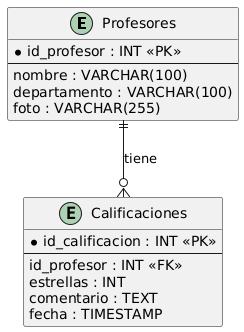
\includegraphics[width=0.4\textwidth]{BD.png}
    \caption{Diseño de la Base de Datos}
\end{figure}

\newpage
\section{Estimación de Costos y Tiempos}

A continuación se presenta una estimación preliminar de los costos y tiempos necesarios para el desarrollo del proyecto \textbf{CalificaProf-UPV}. Estos valores son aproximados y podrán ajustarse conforme se defina el alcance final del proyecto.

\subsection{Estimación de Costos}

La siguiente tabla resume la estimación de horas y costos por cada fase del proyecto:

\begin{center}
\begin{tabular}{lccc}
\toprule
\textbf{Fase} & \textbf{Horas Estimadas} & \textbf{Costo por Hora (USD)} & \textbf{Costo Total (USD)} \\
\midrule
Análisis y Requerimientos       & 40  & \$25 & \$1,000 \\
Diseño UI/UX                   & 80  & \$30 & \$2,400 \\
Desarrollo Frontend            & 120 & \$35 & \$4,200 \\
Desarrollo Backend             & 120 & \$35 & \$4,200 \\
Integración y Testing          & 80  & \$30 & \$2,400 \\
Despliegue                     & 40  & \$25 & \$1,000 \\
Documentación y Capacitación   & 40  & \$25 & \$1,000 \\
\midrule
\textbf{Total}                 & 520 & ---  & \$16,200 \\
\bottomrule
\end{tabular}
\end{center}

\subsection{Estimación de Tiempos}

La siguiente tabla muestra la duración estimada de cada fase en semanas, considerando que algunas fases se realizan de manera secuencial:

\begin{center}
\begin{tabular}{lcc}
\toprule
\textbf{Fase} & \textbf{Duración Estimada (semanas)} & \textbf{Notas} \\
\midrule
Análisis y Requerimientos       & 1 & \\
Diseño UI/UX                   & 2 & \\
Desarrollo Frontend            & 3 & \\
Desarrollo Backend             & 3 & \\
Integración y Testing          & 2 & \\
Despliegue                     & 1 & \\
Documentación y Capacitación   & 1 & \\
\midrule
\textbf{Total}                 & 13 & Duración total estimada \\
\bottomrule
\end{tabular}
\end{center}

\bigskip
\textbf{Observaciones:} \\
Las estimaciones presentadas son preliminares y están sujetas a revisión conforme se avance en la definición de requisitos, alcance y asignación de recursos. Los costos totales pueden variar en función de cambios en la planificación o en el equipo de trabajo.


\end{document}
